\documentclass{article}

% Language setting
% Replace `english' with e.g. `spanish' to change the document language
\usepackage[english]{babel}

% Set page size and margins
% Replace `letterpaper' with `a4paper' for UK/EU standard size
\usepackage[letterpaper,top=2cm,bottom=2cm,left=3cm,right=3cm,marginparwidth=1.75cm]{geometry}

% Useful packages
\usepackage{amsmath}
\usepackage{graphicx}
\usepackage[colorlinks=true, allcolors=blue]{hyperref}

\title{Energy usage prediction}
\date{}
\begin{document}
\maketitle

\begin{abstract}
Accurate building energy consumption forecasting plays an important role in improving energy efficiency, reducing operational costs, and supporting sustainable smart-building management systems. This project predicts hourly building energy consumption using the ASHRAE Great Energy Predictor III dataset, which contains large-scale building metadata, weather data, and meter readings from multiple sites and building types. Preprocessing and feature engineering included missing-value imputation, anomaly handling, logarithmic transformations, lag features, rolling weather statistics, and temporal feature extraction. Linear Regression, Random Forest, XGBoost, LightGBM and CatBoost were trained and evaluated using Root Mean Squared Logarithmic Error (RMSLE). Gradient-boosting models consistently outperformed the linear baseline on this structured tabular task. CatBoost achieved the strongest single-model result with an RMSLE of approximately 0.5022 after hyperparameter tuning, while a soft-voting ensemble of CatBoost and LightGBM achieved the best overall result of 0.4997.

\end{abstract}

\section{Introduction}

Energy efficiency claims are usually settled by comparison rather than by direct measurement. The saving attributed to a retrofit is the difference between observed consumption and the consumption a baseline model would have predicted under the same weather, calendar and operating conditions \cite{miller2020}. The ASHRAE Great Energy Predictor III data set, released for the 2019 Kaggle competition, was assembled with that kind of counterfactual estimation in mind. It pairs hourly meter readings for electricity, chilled water, steam and hot water with static building metadata and with contemporaneous weather observations recorded at sixteen sites.

Modelling these meters is harder than the size of the data alone suggests. Demand depends on building use, gross floor area, hour of day, day of week, season, and recent consumption history, and the interactions between those factors are non-linear. Outdoor temperature has a piecewise effect: a one-degree shift inside the comfort band moves load very little, but the same shift in a heating- or cooling-dominated period changes load substantially. The data themselves carry several documented artefacts. Roughly 60\% of \texttt{year\_built} and 83\% of \texttt{floor\_count} are missing in the metadata. The weather table has station-specific gaps in cloud cover, precipitation, sea-level pressure and wind direction. Site 0 records implausibly low electricity readings before 20 May 2016, and a non-trivial fraction of building-meter pairs show long zero-reading runs that look more like outages than genuine zero load.

The target variable is heavily right-skewed. All models were fitted on \(\log1p(\text{meter\_reading})\) and assessed with RMSLE, since proportional rather than absolute error is the only criterion that places a small office and a large hospital on a comparable footing when consumption volumes span several orders of magnitude.

What follows develops three threads in turn. The ingestion stage joins \texttt{train}, \texttt{building\_metadata} and \texttt{weather\_train} into a single 20,216,100-row table, with every one of the 1,449 building identifiers preserved. The cleaning stage translates the Sprint 1 audit findings into explicit rules on the merged table: Site 0 electricity records before 20 May 2016 and unreliable long-zero building-meter pairs are removed, metadata is imputed at the primary-use level, weather gaps are closed station-by-station before the join, and a coherent set of calendar, lag, rolling, weather-derivative and building-derivative features is engineered. The modelling stage then compares five families (XGBoost, LightGBM, CatBoost, Random Forest and Linear Regression) under a strictly chronological split. January to October 2016 is used for training and November to December 2016 is held out as the test set, so that the short-range temporal autocorrelation of meter readings cannot be exploited by a random split.


\section{Literature Review} 
Recent building energy prediction literature shows that traditional machine learning, especially tree-based ensemble models, is more common than standalone deep learning for structured tabular datasets. The ASHRAE Great Energy Predictor III overview paper reports a large real-world dataset with 1,448 buildings, 2,380 meters and over 20 million training records, evaluated using RMSLE \cite{miller2020}. The top Kaggle solutions mainly relied on ensemble gradient-boosting methods such as LightGBM, XGBoost, and CatBoost, sometimes combined with neural networks \cite{budslab}. This shows that deep learning appeared in some ensembles, but boosting models were central. 

\subsection{Insights from the ASHRAE Great Energy Predictor III Competition}
A detailed analysis of the top-performing teams in the ASHRAE Great Energy Predictor III competition further validates the effectiveness of gradient-boosting approaches and extensive preprocessing for large-scale building energy prediction. The first-place team, Motoki and Yamashita, found that data cleaning and fixing anomalies were the most important factors for model performance. Their solution included removing unusual meter readings, correcting inconsistencies in Site 0 units, filling in missing weather data, adjusting timestamps to local time, and applying a log1p transformation to the target variable. Their final model combined CatBoost, LightGBM, and MLP models trained on various levels of detail using extensive feature engineering. This included lag features, cyclical time encoding, target encoding, and weather smoothing techniques \cite{motoki2020}. The second-place team, cHa0s, also focused on LightGBM and XGBoost models. They emphasized modeling each site separately and highlighted the importance of lag-based features, like weekly lag (\texttt{lag\_168}), and rolling weather statistics \cite{chaos2020}. Similarly, the third-place team, eagle4, showed that averaging several well-validated LightGBM models yielded better results than depending solely on complex neural network structures \cite{eagle42020}. Across the top solutions in the competition, common strategies included thorough data cleaning, log-transformed targets, time-aware evaluation methods, and ensemble learning with gradient-boosting models. 

\subsection{Effectiveness of Gradient-Boosting Methods}
Several papers confirm the strength of boosting methods. Miller et al. found that gradient boosting machines, especially LightGBM, performed best in the ASHRAE competition when combined with preprocessing, imputation and outlier removal \cite{miller2022}. A comparison of LightGBM, XGBoost and CatBoost also showed that boosting models capture nonlinear relationships between weather, building characteristics and energy use effectively \cite{gbmcomparison}. Similarly, an XGBoost quantile regression study compared XGBoost with ANN, SVM and Random Forest, showing that boosting can provide strong accuracy and interpretability through feature-importance methods such as SHAP \cite{xgboostshap}. 


CatBoost-specific studies further support its effectiveness for tabular energy prediction tasks. A CatBoost model tuned using random search and Bayesian optimisation achieved very high accuracy for building energy prediction and outperformed several baseline models \cite{catboostbayes}. Another CatBoost study using meta-heuristic optimisation also showed strong performance on feature-based energy data, although optimisation increased computational cost \cite{qu2026}. Overall, gradient-boosting models such as LightGBM, XGBoost and CatBoost are widely adopted due to their ability to model nonlinear feature interactions and deliver strong performance on structured building energy data.

\section{Methodology}
This project follows an iterative machine learning pipeline inspired by the approaches used in the top-performing solutions of the ASHRAE Great Energy Predictor III competition. The overall workflow of the system is illustrated in figure \ref{fig:pipeline}. The methodology begins with integrating the building metadata, weather, and meter-reading datasets, followed by preprocessing, feature engineering, model training, and evaluation.

\begin{figure}[h]
    \centering
    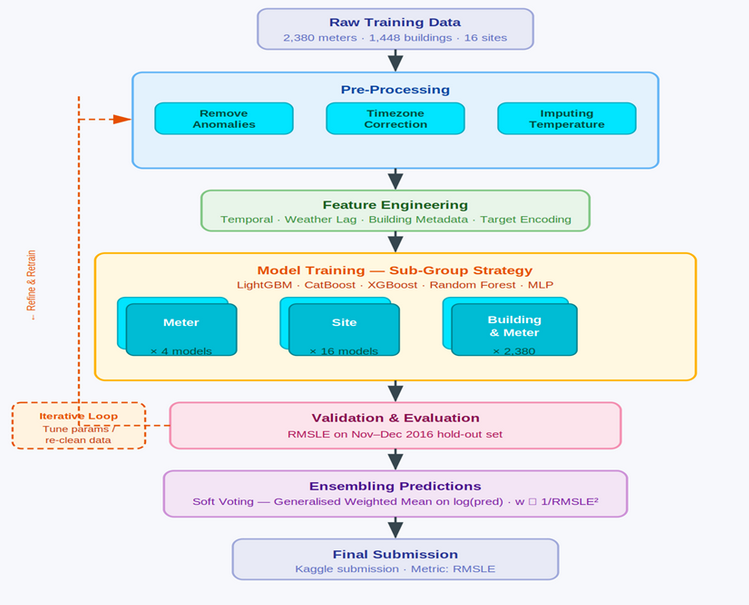
\includegraphics[width=0.75\linewidth]{Pipeline.png}
    \caption{Iterative Model Pipeline}
    \label{fig:pipeline}
\end{figure}

\subsection{Data Preprocessing and Analysis}
\subsubsection{Building Metadata Dataset}

The building metadata dataset contains descriptive information about each building included in the ASHRAE energy prediction dataset. It includes attributes such as building ID, site ID, primary building usage category, square footage, year built, and floor count. It contains data for 1449 buildings. This dataset plays an important role in providing contextual information that helps machine learning models understand how building characteristics influence energy consumption patterns.


\begin{figure}[h]
    \centering
    
\includegraphics[width=0.60\linewidth]{primay_use.png}
    \caption{Primary Use Count Distribution}
    \label{fig:primary_use}
\end{figure}

The dataset represents a diverse collection of buildings distributed across multiple geographic sites[\ref{fig:primary_use}]. The \texttt{site\_id} attribute indicates different weather locations, allowing the integration of local climate information with building-level energy usage. Buildings in the dataset belong to 16 different primary usage categories, including education, office, healthcare, lodging/residential, retail, technology/science, and warehouse/storage. Education had the highest number of buildings, with 549 entries, followed by office buildings with 279 entries. In contrast, fewer than 10 buildings belonged to categories such as Technology/Science, Food Sales and Service, Utility, and Religious Worship. Since these categories are nominal and non-ordinal, One-Hot Encoding was applied to convert them into machine-readable binary features without introducing artificial ordering relationships.


The \texttt{square\_feet} feature showed a highly skewed distribution with a very large size range between small and large buildings[\ref{fig:pic0},\ref{fig:pic2}]. To reduce skewness and stabilize variance, a logarithmic transformation (\texttt{log\_square\_feet}) was applied using the \texttt{log1p()} function. The \texttt{year\_built} feature was used to derive a new attribute called \texttt{building\_age}, calculated relative to the dataset year (2016). This transformation allowed the model to capture the effect of building age more effectively than using raw construction years.

\begin{figure}[h]
    \centering
    
    \begin{minipage}{0.45\linewidth}
        \centering
        
\includegraphics[width=\linewidth]{raw_SF.png}
        \caption{Raw Square Feet Distribution}
        \label{fig:pic0}
    \end{minipage}
    \hfill
    \begin{minipage}{0.45\linewidth}
        \centering
        
\includegraphics[width=\linewidth]{engi_SF.png}
        \caption{Log1p Transformed Square Feet}
        \label{fig:pic2}
    \end{minipage}
    
\end{figure}

Several missing-data handling decisions were made during preprocessing. The \texttt{floor\_count} attribute contained a large proportion of missing values; however, instead of removing the feature entirely, a new binary feature called \texttt{missing\_floor\_count\_flag} was created to preserve information about missingness. Missing floor counts were then imputed using grouped median values based on \texttt{primary\_use}, \texttt{site\_id}, and building-size categories derived from square footage. Missing \texttt{year\_built} values were similarly imputed using grouped medians by building type and site. These decisions were made to retain potentially useful structural information while minimizing information loss and maintaining dataset consistency for model training.


\subsubsection{Weather Dataset}

Weather data were cleaned before merging because each station-hour reading is shared by all buildings at the same site. Imputing after the join would duplicate one missing station reading across many building rows and distort fill statistics. Therefore, \texttt{weather\_train.csv} and \texttt{weather\_test.csv} were sorted by \texttt{site\_id} and \texttt{timestamp}, processed using the same station-level preprocessing function, and then joined to the meter data. The training merge preserved all 20,216,100 rows, confirming that missingness originated from the weather variables rather than from the join itself.

\begin{figure}[h]
    \centering
    
\includegraphics[width=0.75\linewidth]{weather1.png}
    \caption{Air Temperature by Timestamp for the First Four Sites in \texttt{weather\_train.csv}}
    \label{fig:weather_air_temp}
\end{figure}

The main missing-value gaps were found in \texttt{cloud\_coverage} (approximately 44\%), \texttt{precip\_depth\_1\_hr} (approximately 19\%), \texttt{wind\_direction} (approximately 7\%), and \texttt{sea\_level\_pressure} (approximately 6\%). In contrast, temperature and wind-speed variables were mostly complete. Gradual variables such as \texttt{air\_temperature} and \texttt{dew\_temperature} were linearly interpolated within each site. The \texttt{cloud\_coverage} feature was forward-filled and backward-filled before applying site-level and global median fallback values. \texttt{precip\_depth\_1\_hr} was filled with zero and paired with a missingness indicator feature. \texttt{sea\_level\_pressure}, \texttt{wind\_direction}, and remaining weather nulls were handled using local rolling medians, site-level medians, and final forward/backward filling.

Two additional weather features were engineered after imputation. The first was \texttt{relative\_humidity}, computed from air temperature and dew temperature and clipped to the valid range of 0--100\%. The second was \texttt{temp\_diff\_from\_comfort}, defined as the absolute difference from a 21$^\circ$C reference temperature. Processed floating-point weather columns were cast to \texttt{float32} before the large train and test merges to reduce memory usage without affecting the precision of tree-based regression models.

After combining the cleaned weather streams with the building-meter data and applying anomaly cleaning, the usable 2016 modelling table contained 17,489,805 rows. A chronological split was applied using January to October 2016 for training and November to December 2016 as the held-out test set. This avoided placing adjacent readings from the same building-meter pair into both datasets and more accurately reflected future-period prediction.

\subsubsection{Train Dataset}
The training dataset contains over 20 million hourly energy readings from 1,441 buildings across four meter types: electricity (0), chilled water (1), steam (2), and hot water (3), covering the year 2016. The dataset includes four primary columns: building\_id, meter, timestamp, and meter\_reading. No missing values were observed in these columns; however, exploratory analysis revealed data quality issues such as skewed distributions and anomalous zero readings that required further processing. 

Energy consumption exhibits clear daily patterns, with peak usage typically occurring during working hours (approximately 12 PM to 4 PM) and lower consumption during night hours. This reflects building occupancy and operational schedules. These patterns justify the inclusion of time-based features such as hour and business-hour indicators.
Energy usage varies significantly across seasons as well. Chilled water demand increases in warmer periods due to cooling requirements, while steam usage is higher in colder periods due to heating demand. This highlights the importance of seasonal features such as month and season in capturing energy consumption behaviour. 

\begin{figure}[h]
    \centering
    
\includegraphics[width=0.60\linewidth]{Test3.png}
    \caption{Average Energy by Month for each meter type}
    \label{fig:test3}
\end{figure}

Energy consumption is consistently higher on weekdays compared to weekends, reflecting reduced building activity during non-working days. This supports the inclusion of a weekend indicator feature to capture operational differences.

\begin{figure}[h]
    \centering
    
\includegraphics[width=0.60\linewidth]{Test4.png}
    \caption{Weekday vs Weekend Comparison for each meter type}
    \label{fig:test4}
\end{figure}

Feature engineering focused on capturing temporal patterns and dependencies in energy consumption. Time-based features such as hour, day\_of\_week, month, and season were extracted from timestamps to represent daily and seasonal variations.
To model historical dependencies, lag features (lag\_24h, lag\_72h, and lag\_168h) were created, capturing consumption from the previous day, three days prior, and one week prior. These features reflect the strong temporal continuity in energy usage.
Additionally, rolling statistics were computed to capture local trends, including 24-hour and 7-day moving averages and standard deviations. A forward shift was applied to prevent data leakage, ensuring that only past information was used. Together, these features enable the model to learn both short-term fluctuations and longer-term consumption patterns.

The distribution of meter readings was highly right-skewed, with most values concentrated at lower levels and a small number of extreme values, particularly for steam meters. To address this, a log transformation (log1p) was applied to stabilise variance and improve model performance, aligning with the RMSLE evaluation metric.
Further investigation identified a large number of zero readings. While many zeros represent valid periods of low or no energy consumption, anomalies were detected in Site 0 electricity data between January and May 2016, where approximately 93.75\% of readings were zero, including long consecutive sequences. This indicated sensor or data collection issues. As a result, all Site 0 electricity data prior to 20 May 2016 was removed. Additionally, building-meter combinations exhibiting continuous zero readings for more than 168 hours were excluded, as these were considered unreliable.
A time-based train-test split was applied, with data from January to October 2016 used for training and November to December reserved for testing. Lag and rolling features were then generated separately within each split, grouped by \texttt{building\_id} and \texttt{meter}; rolling windows used \texttt{shift(1)} so each feature depended only on earlier readings.



\subsection{Model Choices \& Justification}

Three gradient-boosted tree models and one bagging ensemble were selected: LightGBM , XGBoost, CatBoost, and Random Forest. A Linear Regression baseline was included as well for comparison. 

The choice of gradient-boosted trees is directly validated by the ASHRAE Great Energy Predictor III competition itself. Miller et al.~\cite{miller2020} reported that the most accurate workflows used large ensembles of gradient-boosting models, with LightGBM dominating many top-performing solutions. The BUDS Lab summary of the competition further showed that all top-5 solutions incorporated LightGBM and/or CatBoost as primary models~\cite{budslab}.

LightGBM was selected because of its leaf-wise tree growth strategy, histogram-based splitting, and computational efficiency when handling very large datasets. Miller, Liu, and Fu also demonstrated that LightGBM-based pipelines combined with careful preprocessing and feature engineering achieved state-of-the-art performance in the competition~\cite{miller2022}. CatBoost was additionally selected because of its ordered boosting strategy and strong handling of categorical variables, which is particularly useful for the 16 one-hot encoded primary-use categories. This choice is supported by both the IEEE Bayesian optimisation study~\cite{catboostbayes} and the CatBoost meta-heuristic forecasting work by Qu and Liu~\cite{qu2026}.

XGBoost uses depth-wise tree growth, producing prediction patterns that differ slightly from LightGBM and therefore providing useful ensemble diversity. Comparative studies of boosting methods and XGBoost quantile regression approaches showed that XGBoost performs strongly for nonlinear building-energy forecasting tasks while also supporting interpretability through feature-importance analysis~\cite{gbmcomparison,xgboostshap}. Random Forest was included as a lower-correlation bagging-based alternative, where independently trained trees help reduce ensemble variance compared to purely boosted approaches.
\subsection{Loss Function \& Optimisation Target}

All models were trained on the log1p-transformed target (\texttt{log\_meter\_reading}) to directly align training with the RMSLE evaluation metric. CatBoost used an explicit \texttt{loss\_function='RMSE'} on the log-scale target. LightGBM and XGBoost used the default squared-error loss on the same transformed target. Random Forest minimises mean squared error natively. Predictions are converted back to the original scale via \texttt{np.expm1()} before evaluation.


\subsection{Evaluation Metric}
Submissions are scored on \textbf{Root Mean Squared Log Error (RMSLE)}:

\[
\text{RMSLE} = \sqrt{\frac{1}{n} \sum_{i=1}^{n} \left( \log(\hat{y}_i + 1) - \log(y_i + 1) \right)^2 }
\]

RMSLE penalises under-predictions more than over-predictions on a multiplicative scale, making it appropriate for meter readings that span several orders of magnitude. A custom \texttt{rmsle()} function is used consistently across all notebooks for fair model comparison.

\subsection{Anomaly Removal}
The final integrated pipeline applied two anomaly-cleaning rules to the 2016 meter data before the train-test split. First, electricity readings from Site 0 before 2016-05-20 were removed because this period had a known unit inconsistency and an abnormal concentration of zero readings. Second, building-meter pairs containing zero-reading streaks longer than 168 hours were excluded, since these sustained flat-zero periods were more consistent with sensor outages or inactive meters than genuine consumption. Additional audits flagged 99.9th-percentile extremes and sudden jumps above ten times the previous non-zero hourly reading, but these were kept as diagnostic findings rather than final removal rules.


\section{Results}

Five model families were compared on the held-out November-December test set: LightGBM, XGBoost, CatBoost, Random Forest, and Linear Regression. The strongest single-model result in the project comes from the tuned CatBoost model, which achieved an overall RMSLE of 0.5022. This outperformed LightGBM at 0.5084, XGBoost at 0.5210, Random Forest (depth=20) at 0.5266, and Linear Regression at 1.5989.

\begin{table*}[h]
\centering
\label{tab:meter_comparison}
\begin{tabular}{|l|c|c|c|c|c|}
\hline
\textbf{Model} & \textbf{Electricity} & \textbf{Chilled Water} & \textbf{Steam} & \textbf{Hot Water} & \textbf{Overall} \\
\hline
CatBoost & 0.2433 & 0.6576 & 0.7098 & 1.0780 & 0.5022 \\
LightGBM & 0.2436 & 0.6623 & 0.7298 & 1.0857 & 0.5084 \\
XGBoost & 0.2612 & 0.6896 & 0.7297 & 1.0927 & 0.5210 \\
Random Forest (depth=20) & 0.2599 & 0.7090 & 0.7315 & 1.1012 & 0.5266 \\
Linear Regression & 0.9970 & 2.1877 & 2.3859 & 2.1438 & 1.5989 \\
\hline
\end{tabular}
\caption{Per-Meter RMSLE Comparison}
\end{table*}


Performance also varied by meter type. For Electricity, tuned CatBoost was best with 0.2433, followed very closely by LightGBM at 0.2436; XGBoost and Random Forest were higher at 0.2612 and 0.2599 respectively. For Chilled Water, CatBoost again led at 0.6576, with LightGBM at 0.6623, XGBoost at 0.6896, and Random Forest at 0.7090. For Steam, CatBoost achieved the lowest RMSLE at 0.7098, ahead of XGBoost at 0.7297, LightGBM at 0.7298, and Random Forest at 0.7315. For Hot Water, the order was the same: CatBoost 1.0780, LightGBM 1.0857, XGBoost 1.0927, and Random Forest 1.1012.

Linear Regression performed much worse across every meter category, especially for Chilled Water and Steam, where RMSLE values were above 2.0.

Overall, the results show that ensemble tree models are the most reliable approach for this dataset, with tuned CatBoost as the strongest single model and LightGBM / XGBoost as close, stable alternatives.


\subsection{Ensemble Methods}
To further improve predictive performance, ensemble methods were explored using both soft and hard voting approaches. Soft voting assigns weights to models based on their performance, allowing stronger models such as CatBoost and LightGBM to contribute more to the final prediction.
The results show that the best soft voting configuration, combining CatBoost and LightGBM, achieved the lowest RMSLE of 0.4997, outperforming all individual models. In contrast, including additional models such as Random Forest and Linear Regression reduced performance, demonstrating that weaker models can negatively impact ensemble results.
Compared to hard voting, soft voting consistently achieved better performance, highlighting the importance of weighted model combination in improving predictive accuracy.

\begin{figure}[h]
    \centering
    
\includegraphics[width=0.75\linewidth]{actual_vs_predicted_sv2_hv2.png}
    \caption{Hard Voting vs. Soft Voting}
    \label{fig:pic3}
\end{figure}


\section{Discussion}
Across LightGBM, XGBoost, CatBoost and Random Forest, error was consistently lowest for electricity (meter 0) with per-meter RMSLE near 0.24--0.26, followed by chilled water (meter 1) and steam (meter 2) in the 0.65--0.74 range, while hot water (meter 3) was the hardest at roughly 1.07--1.11. The same ranking held across all tree models, indicating the difficulty is data-driven rather than model-specific.

\begin{figure}[h]
    \centering
    
\includegraphics[width=0.75\linewidth]{rmsle_per_meter_type_all_models.png}
    \caption{Per Meter RMSLE of the Boosting Models}
    \label{fig:pic1}
\end{figure}



\subsection{Comparison to Baseline Linear Regression}
Linear Regression achieved a test RMSLE of 1.5989 and the median baseline 1.3254, whereas the best individual model (CatBoost) reached 0.5022 and the ensemble methods improved further. This represents an approximately 68\% reduction in RMSLE over linear regression, demonstrating that the meter, weather and calendar relationship is strongly non-linear and interaction-heavy, which gradient-boosted trees capture but a linear model cannot.

\subsection{Possible Reasons Why Electricity Was More Accurate Than Hot Water}
Electricity is metered in every building and follows highly regular daily and weekly occupancy cycles, giving the boosted trees strong, repeatable signals from hour, is\_business\_hours and the lag features. Hot water, in contrast, is installed in far fewer buildings, is dominated by intermittent and weather-driven demand, contains long zero-streaks, and shows abrupt seasonal switching, all of which weaken temporal regularity and inflate log-scale errors.

\subsection{Impact of Site 0 Anomaly Removal}
Removing Site 0 electricity readings before 2016-05-20 (kBTU vs kWh unit inconsistency) and excluding long zero-streak building-meter pairs produced the largest data-cleaning gain. Before cleaning, Site 0 alone contributed disproportionately to squared log error; afterwards, test RMSLE improved across the tree models and the per-site error distribution became more uniform, confirming that the main issue was label quality rather than model capacity.

\subsection{Where Lag Features Helped Most}
The lag\_24h, lag\_168h and rolling\_mean\_24h features ranked among the top-five LightGBM and XGBoost importances[\ref{fig:feat_imp}]. Their benefit was greatest for electricity and chilled water, where consumption is strongly auto-correlated on daily and weekly cycles. Gains were smaller for steam and hot water, whose readings are sparser and more weather-shock driven, so recent history is a weaker predictor of the next hour.

\begin{figure}[h]
    \centering
    
\includegraphics[width=0.75\linewidth]{feat_imp.png}
    \caption{Top 15 Feature Importance}
    \label{fig:feat_imp}
\end{figure}


\subsection{Hyperparameter Tuning}
Because the full dataset was computationally expensive, hyperparameter search was run on random samples from the January-October training split only. LightGBM used 15 \texttt{RandomizedSearchCV} trials with 3-fold cross-validation on 30\% of the training split; the selected parameters were \texttt{n\_estimators=1500}, \texttt{learning\_rate=0.07}, \texttt{num\_leaves=127}, \texttt{min\_child\_samples=50}, and \texttt{reg\_alpha=1.0}. CatBoost used 12 trials with 3-fold cross-validation on 20\% of the training split; the selected parameters were \texttt{iterations=1500}, \texttt{learning\_rate=0.07}, \texttt{depth=8}, \texttt{l2\_leaf\_reg=3}, and \texttt{border\_count=254}. XGBoost and Random Forest used smaller 2-fold searches on 5\% samples because of longer training times. The selected LightGBM and CatBoost models were refit on the full training split and evaluated once on the held-out test set.

\subsection{Ensemble Weighting}
Both Hard Voting and Soft Voting were evaluated using different variations of LightGBM, XGBoost, CatBoost, Random Forest and Linear Regression. Out of all of them, Soft Voting using the best two models, CatBoost and LightGBM achieved the best ensemble RMSLE[\ref{fig:ensemble}].

\begin{figure}[h]
    \centering
    
\includegraphics[width=0.75\linewidth]{ensemble_comparison.png}
    \caption{Hard Voting vs. Soft Voting}
    \label{fig:ensemble}
\end{figure}

\subsection{Error Analysis}
Residual inspection showed errors are not uniformly distributed: the largest log-residuals concentrate on (i) very low or zero readings that the model slightly over-predicts, (ii) extreme summer-peak steam and hot-water spikes that are under-predicted, and (iii) buildings with short training history. RMSLE also penalises under-prediction more heavily than over-prediction, which amplifies the visible error on peak hot-water hours. Errors were near-zero-mean per building but heavy-tailed, consistent with sensor noise and unmodelled occupancy events.


\section{Limitations}
Despite showing promising results, the project has several limitations. First, the best model reached an RMSLE of approximately 0.4997, which leaves room for further improvement on difficult meters such as hot water. Second, the dataset created significant computational challenges: the raw merged table had over 20 million rows, and the final feature set contained 49 variables after time, weather, building and lag/rolling features were added. Training on the complete dataset required substantial memory and processing time. Only two of the six team members could train the largest models locally, and even Google Colab Enterprise struggled with the final processed dataset. Because of these constraints, the project could not exhaustively test every preprocessing choice, feature variant, or hyperparameter combination.

\section{Future Work}
To further enhance the performance and robustness of the system, several improvements can be explored in the future. More advanced feature engineering techniques, particularly building-specific temporal features and seasonal trend analysis, could improve the model's ability to capture long-term consumption behavior. Extensive hyperparameter optimization using automated search methods such as Grid Search, Random Search, or Bayesian Optimization may also lead to better predictive performance. Additionally, transformer-based or recurrent deep learning architectures designed for time-series forecasting can be explored. Using more powerful computational resources would allow for more extensive experimentation. Finally, incorporating external contextual information such as holidays, occupancy patterns, or regional energy usage trends may help improve prediction accuracy and model generalization.

\section{Conclusion}
Overall, the project shows that reliable energy prediction depends as much on careful preparation as on model choice. Joining the meter, building and weather data created a complete modelling table, while the main cleaning decisions removed known calibration and outage artefacts before feature engineering. Handling metadata and weather gaps consistently also made the inputs more comparable across buildings, sites and time.
The strongest results came from tree-based methods, with a small additional gain from a weighted ensemble. This supports the use of flexible non-linear learners for hourly building-energy data, but it also shows that well-structured features and chronological test evaluation are central to fair comparison. Future work should test robustness over later periods, compare errors by site and meter type, and explore stacking only after data quality and leakage controls are secured.


\bibliographystyle{IEEEtran} 
\bibliography{references}

\end{document}
